\chapter{Algoritmo de detección}
\label{Ch:4}
\graphicspath{{figs/}}
%%%%%%%%%%%%%%%%%%%%%%%%%%%%%%%%%%%%%%%%%%%%%%%%%%%%%%%%%%%%%%%%%%%%%%%%

En este capítulo se trata el problema de detección, el cual es fundamental resolver para el funcionamiento de los algoritmos de sincronismo implementados. La correcta detección de una señal entrante indica en qué instante uno debe \color{Green} aplicar \color{black} los algoritmos de sincronismo definidos e implementados en el Capítulo \ref{Ch:3}. 

La primera parte de este capítulo se centra en la formalización de una prueba de hipótesis que determinará si un registro de datos bajo prueba contiene una señal de interés. Se estudian las propiedades estadísticas del ruido y de una señal afectada por el mismo, y en función de estas propiedades se formaliza una regla de decisión. En la segunda parte se trata el problema de la estimación de la varianza del ruido, ya que conocerla es necesario para la correcta aplicación de la regla de decisión definida.

\section{Prueba de hipótesis}
\label{S:prueba-hipotesis}

El problema de detección se resolverá por medio de una prueba de hipótesis sobre las muestras de una señal presentes en una ventana de recepción, agrupadas en el vector
\begin{equation}\label{eq:def_y}
    \mathbf{y} = \begin{bmatrix}
        y[0] & y[1] & \cdots & y[N-1]
    \end{bmatrix},
\end{equation}
donde $N$ coincide con la longitud de la secuencia de entrenamiento de símbolos cortos. 

Los pasos para realizar la prueba son los siguientes:
\begin{enumerate}
    \item definición de dos o más hipótesis mutuamente excluyentes acerca del origen de las muestras observadas;
    \item definición de un estadístico en función de las muestras bajo estudio, que recibe el nombre $\phi\left[\mathbf{y}\right]$;
    \item definición de una regla de decisión sobre el estadístico elegido para discriminar entre las hipótesis disponibles según determinado criterio;
    \item estimación de los parámetros necesarios para aplicar la regla de decisión.
\end{enumerate}

\subsection{Definición de hipótesis}
\label{Ss:def-hipotesis}

Se definen dos hipótesis sobre la composición de las muestras, estas reciben el nombre de hipótesis nula ($H_0$) e hipótesis alternativa ($H_1$), y son las siguientes:
\begin{itemize}
    \item $H_0$: el intervalo de evaluación contiene únicamente ruido;
    \item $H_1$: el intervalo de evaluación contiene una secuencia de entrenamiento de símbolos cortos afectada por ruido aditivo y modificada por el canal inalámbrico.
\end{itemize}

Se hacen varias suposiciones en las definiciónes de las hipótesis:
\begin{enumerate}
    \item las muestras de ruido siguen la distribución normal compleja, son independientes, e idénticamente distribuidas;
    \item la respuesta al impulso del canal puede ser aproximada por un único \textit{tap}, por lo que cada muestra de la secuencia transmitida se ve modificada por un factor de amplitud y fase, pero no influye a las muestras anteriores ni a las siguientes;
    \item el canal presenta desvanecimiento lento, por lo que el factor que modifica la amplitud y fase de una señal recibida se mantiene aproximadamente constante.
\end{enumerate}
\color{Green}
La primera y tercera de estas suposiciones son consistentes con los modelos de canales inalámbricos utilizados en la práctica, pero la segunda suposición implica una sobresimplificación del modelo del canal para los propósitos del desarrollo del algoritmo de detección, ya que OFDM se utiliza en canales selectivos en frecuencia los cuales tienen respuestas al impulso de múltiples taps \cite{tse}. Sin embargo, estudios previos realizados por el grupo sobre OFDM concluyen que éste modelo es viáble para la detección incluso cuando la respuesta al impulso del canal es selectiva en frecuencia \cite{tesis-daniel}. \color{black} Tomando en cuenta las suposiciones, se procede a formalizar las expresiones matemáticas de las hipótesis;
\begin{equation}\label{eq:def-hipótesis}
    \begin{aligned}
        H_0&: \quad \mathbf{y} = \mathbf{w}\\
        H_1&: \quad \mathbf{y} = A\mathbf{s} + \mathbf{w}
    \end{aligned}
    \qquad\qquad
    \mathbf{w} \sim \mathcal{CN}\left[\mathbf{0},\, \sigma^2 I_N\right],
\end{equation}
donde $\mathbf{s}$ es la secuencia de entrenamiento de símbolos cortos, de $N$ muestras de longitud, y $A$ es un factor complejo desconocido, pero constante, que modifica la amplitud y fase de la secuencia. 

\subsubsection{Definición de SNR}
\label{Ss:def-snr}

En el caso de que la hipótesis alternativa sea verdadera, resulta conveniente definir una medida de la relación señal a ruido. La definición utilizada es el cociente entre la potencia media de una muestra de señal y la potencia media de una muestra de ruido
\begin{equation}\label{eq:snr-definicion}
\text{SNR} = \frac{\text{Potencia media señal}}{\text{Potencia media ruido}}.
\end{equation}

Las suposiciones hechas implican que la potencia media de la señal es un valor determinístico, dado por
\begin{equation}\label{eq:potencia-señal}
\overline{P}_s = \frac{1}{N}\sum_{k=0}^{N-1}\lvert A s[k] \rvert^2 = \frac{1}{N} \lvert A \rvert^2 \lVert \mathbf{s} \rVert^2,
\end{equation}
mientras que la potencia media del ruido surge de las propiedades estadísticas de su distribución, y se calcula a partir de la propiedad del módulo de una variable aleatoria normal compleja, el cual sigue una distribución Rayleigh
\begin{equation}
w[k] \sim \mathcal{CN}\left[0, \sigma^2\right]  \implies|w[k]| \sim \mathcal{R}ay\left[\sigma\right],
\end{equation}
y el hecho de que media de la distribución Rayleigh es conocida, así como lo es su varianza
\begin{equation}
E\left[\lvert w[k]\rvert\right] = \sigma \sqrt{\frac{\pi}{2}}\qquad\qquad V[\left\lvert w[k] \rvert\right] = \frac{4-\pi}{2} \sigma^2,
\end{equation}
lo cual permite calcular la potencia media de una muestra de ruido de la siguiente forma
\begin{equation}\label{eq:potencia-ruido}
    E\left[\lvert w[k]\rvert^2\right] = V\left[\lvert w[k]\rvert\right] + E\left[\lvert w[k]\rvert\right]^2 =  2\sigma^2.
\end{equation}

Remplazando los valores obtenidos de las Ecuaciones \ref{eq:potencia-señal} y \ref{eq:potencia-ruido} en la Ecuación \ref{eq:snr-definicion} se obtiene la expresión de la SNR presente cuando la hipótesis alternativa es verdadera,
\begin{equation}
\text{SNR} = \frac{\lvert A\rvert^2 \lVert \mathbf{s} \rVert ^2}{2N \sigma^2}.
\end{equation}

\subsection{Elección de estadístico de detección}
\label{Ss:hipotesis-estadistico}

\color{Green}
Se decide utilizar como estadístico de detección el móodulo de la correlación con la secuencia de entrenamiento de símbolos cortos, la cual ha sido estudiada ya que es la base del algoritmo de sincronismo con banco de correladores,
\begin{equation}
    \phi[\mathbf{y}] = \left\lvert\sum_{k=0}^{N-1} s^\ast[k]y[k]\right\rvert = \lvert \mathbf{s}^\ast\mathbf{y}\rvert.
\end{equation}
El motivo de esta elección se basa en que dicho estadistico coincide con un aproximación del estadístico óptimo según el criterio de Neyman-Pearson cuando la señal de interés se encuentra afectada por un modelo de ruido aditivo gausiano \cite{richards}. Esta aproximación asegura la tratabilidad matemática al utilizar un resultado intermedio que es lineal en función de las muestras,
\begin{equation}
    \psi[\mathbf{y}] = \sum_{k=0}^{N-1} s^\ast[k]y[k] = \mathbf{s}^\ast\mathbf{y}.
\end{equation}

Mientras que el funcional del método \textit{delay and correlate} también está disponible para la utilización como estadístico de detección, la presencia de productos de muestras afectadas por el ruido en su expresión implica operaciones no lineales de variables aleatorias, las cuales dificultan la obteción de expresiones cerradas para la distribución del estadístico de detección.
\color{black}

\subsection{Distribución del estadístico ante hipótesis nula}

Se estudia la distribución del \color{Green}resultado intermedio \color{black} $\psi$ en el caso que $\mathbf{y}$ posee únicamente la contribución del ruido,
\begin{equation}\label{eq:psi-ante-h0}
    \mathbf{y} | H_0 = \mathbf{w} \implies \psi[\mathbf{y}] | H_0= \sum_{k = 0}^{N-1} s^\ast[k]w[k].
\end{equation}

En estas condiciones, se observa que $\psi$ resulta una sumatoria de muestras de ruido, cada muestra escalada por su correspondiente término de la secuencia de entrenamiento de símbolos cortos. Esto resulta en una sumatoria de variables normales complejas independientes de diferente varianza. La distribución de cada término de la sumatoria, $z[k] = s^\ast[k]w[k]$, es la siguiente:
\begin{equation}
    z[k] \sim \mathcal{CN}[0,\, \lvert s[k]\rvert^2\sigma^2].
\end{equation}

A partir de la distribución de los términos, la distribución de la sumatoria se calcula con las propiedades de la suma de variables aleatorias gaussianas independientes, y se reduce a la siguiente expresión:
\begin{equation}
    \begin{aligned}
        \psi | H_0 &\sim \mathcal{CN}\left[0,\, \sum_{k=0}^{N-1} \lvert s[k]\rvert^2  \sigma^2 \right],\\[0.5em]
        \psi | H_0 &\sim \mathcal{CN}\left[0,\,\lVert \mathbf{s}\rVert^2  \sigma^2 \right].
    \end{aligned}
\end{equation}

Al igual que se ha visto en la Sección \ref{Ss:def-snr}, el módulo de una distribución normal compleja sigue una distribución Rayleigh, por lo que se conoce la distribución de $\phi$ condicionada por $H_0$. La expresión de su distribución acumulada resulta
\begin{equation}\label{eq:phi-ante-h0}
    F_\phi(\phi|H_0) = 1- \exp\left[-\frac{\phi^2}{2\lVert\mathbf{s}\rVert^2 \sigma^2}\right].
\end{equation}

\subsection{Distribución del estadístico ante hipótesis alternativa}

Nuevamente, se parte de la distribución de $\psi$, en este caso cuando la hipótesis alternativa es verdadera,
\begin{equation}\label{eq:psi-ante-h1}
    \begin{aligned} 
        \mathbf{y} | H_! = A\mathbf{s} + \mathbf{w} \implies \psi[\mathbf{y}] | H_1  
        &= \mathbf{s}^\ast\left(A\mathbf{s}+\mathbf{w}\right)\\ 
        &= A\lVert\mathbf{s}\rVert^2+\mathbf{s}^\ast\mathbf{w}.
    \end{aligned}
\end{equation}

Es evidente la similitud de este caso con el estudiado anteriormente. La Ecuación \ref{eq:psi-ante-h1} describe la suma de un término determinístico y un término aleatorio, el efecto del término determinístico es únicamente el de desplazar la media de la distribución, obteniendo
\begin{equation}
    \psi | H_1 \sim \mathcal{CN}\left[A\lVert\mathbf{s}\rVert^2,\,\lVert \mathbf{s}\rVert^2  \sigma^2 \right].
\end{equation}

Nuevamente, $\psi$ sigue una distribución normal compleja, pero en este caso ya no es de media nula. Para proceder se normaliza la variable aleatoria, definiendo una nueva variable aleatoria $\psi'$ con varianza unitaria,
\begin{equation}
    \psi' = \frac{\psi}{\lVert \mathbf{s} \rVert \sigma} \quad \implies \quad     \psi' | H_1 \sim \mathcal{CN}\left[\frac{A\lVert\mathbf{s}\rVert}{\sigma},\, 2 \right],
\end{equation}
y con el mismo factor de normalización se define la variable $\phi'$, la cual comparte con $\psi'$ la misma relación que sus respectivas equivalentes no normalizadas:
\begin{equation}
\phi' = \frac{\phi}{\lVert \mathbf{s} \rVert \sigma} \quad \longrightarrow \quad     \phi' = \lvert\psi'\rvert.
\end{equation}

El propósito de la normalización es que ésta permite utilizar la definición de la distribución $\chi$ no central \cite{distributions}, la cual es definida de la siguiente forma: si existen $n$ variables aleatorias normales $x_i$ independientes de varianza unitaria y respectivas medias $\mu_i$, y se define $z$ como la raíz de la sumatoria de sus cuadrados
\begin{equation}
    z = \sqrt{\sum_{i=1}^{n}x_i^2},
\end{equation}
ésta variable seguirá la distribución $\chi$ no central de $n$ grados de libertad y parámetro de no-centralidad $\lambda$, el cual es calculado de la siguiente forma
\begin{equation}
    \lambda = \sqrt{\sum_{i=1}^{n}\mu_i^2}.
\end{equation}

Esta definición permite encontrar la distribución de $\phi'$, en tal caso se tiene $n = 2$ grados de libertad, $x_1$ y $x_2$ son la parte real e imaginaria de $\psi'$ respectivamente, y $\mu_1$ y $\mu_2$ son la parte real e imaginaria de su media compleja. Se obtiene el parámetro $\lambda$
\begin{equation}
    \displaystyle\mu_1 = \frac{\rVert\mathbf{s}\rVert}{\sigma}\mathcal{R}e\left[A\right] \quad \displaystyle\mu_2 = \frac{\rVert\mathbf{s}\rVert}{\sigma}\mathcal{I}m\left[A\right] \quad \implies \quad \lambda = \frac{\lVert\mathbf{s}\rVert}{\sigma}\lvert A \rvert
\end{equation}

Resulta la distribución
\begin{equation}
    \phi' | H_1 \sim \chi_{NC}\left[n = 2, \, \lambda = \frac{|A|\lVert\mathbf{s}\rVert}{\sigma}\right] 
\end{equation}

Tal como se hizo en el caso anterior, se continúa trabajando con la función de probabilidad acumulada, la cual en esta oportunidad está dada por
\begin{equation}
    F_{\phi'}(\phi'|H_1) = 1-\int_{\phi'}^\infty x\exp\left[-\frac{x^2 + \frac{|A|^2\lVert\mathbf{s}\rVert^2}{\sigma^2}}{2}\right]I_0\left[\frac{|A|\lVert\mathbf{s}\rVert}{\sigma} x\right] dx,
\end{equation}
en donde $I_n[z]$ es la función de Bessel modificada de primera especie. 

Finalmente, se aplica el cambio de variables para revertir la normalización, obteniendo la distribución acumulada de $\phi$ condicionada por la hipótesis alternativa
\begin{equation}\label{eq:phi-ante-h1}
    F_\phi(\phi|H_1) = 1-\int_{\frac{\phi}{\lVert\mathbf{s}\rVert\sigma}}^\infty x\exp\left[-\frac{x^2 + \frac{|A|^2\lVert\mathbf{s}\rVert^2}{\sigma^2}}{2}\right]I_0\left[\frac{|A|\lVert\mathbf{s}\rVert}{\sigma} x\right] dx.
\end{equation}


\subsection{Regla de decisión}
\label{Ss:hipotesis-umbral}\label{eq:def-pfa}

La regla de decisión típica en los casos que se cuentan con dos hipótesis es la comparación del estadístico con un umbral $T$, tal que si el estadístico excede el umbral se decide por la hipótesis alternativa, mientras que si no lo hace se opta por la hipótesis nula,
\begin{equation}
    \phi[\mathbf{y}]\mathop{\lessgtr}_{H_1}^{H_0}T.
\end{equation}

En función del estadístico y el umbral se definen la probabilidad de falsa alarma, $P_{FA}$, que es la probabilidad de decidir por la hipótesis alternativa cuando la hipótesis nula es verdadera.
\begin{equation}
    P_{FA} = \int_T^\infty f_\phi(\phi|H_0)d\phi = 1 - F_\phi(T|H_0)
\end{equation}

Asimismo, se define la probabilidad de eetección, $P_D$, la cual es la probabilidad de decidir por la hipótesis alternativa cuando esta efectivamente es verdadera.
\begin{equation}\label{eq:probabilidad-deteccion-def}
    P_{D} = \int_T^\infty f_\phi(\phi|H_1)d\phi = 1 - F_\phi(T|H_1)
\end{equation}

El criterio elegido para la elección del umbral es tal que la probabilidad de falsa alarma se mantenga constante a un valor elegido. Tomando la expresión de $F_\phi(\phi|H_0)$ calculado en la Ecuación \ref{eq:phi-ante-h0}, y remplazándolo en la Ecuación \ref{eq:def-pfa} se obtiene
\begin{equation}
    P_{FA} = \exp\left[-\frac{T^2}{2\lVert\mathbf{s}\rVert^2 \sigma^2}\right],    
\end{equation}
y despejando $T$ surge la función para determinar el umbral que obtendrá la probabilidad de falsa alarma deseada,
\begin{equation}\label{eq:umbral}
    T(P_{FA}) = \sqrt{-2\lVert \mathbf{s}\rVert^2 \sigma^2 \ln\left[P_{FA}\right]}.
\end{equation}

\begin{figure}[t]
    \centering{}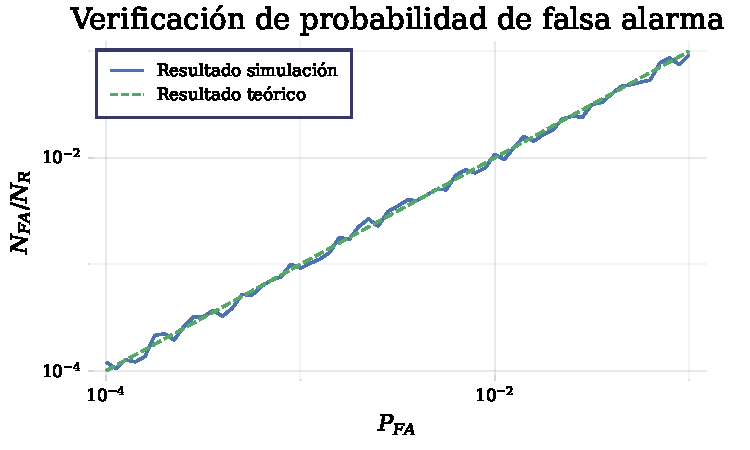
\includegraphics[width=\imsize]{pfa_test.pdf}
    \caption{Resultados de simulación para verificar la correcta probabilidad de falsa alarma de la regla de decisión.\label{fig:pfa-test}}  
\end{figure}

El correcto funcionamiento del umbral para el criterio elegido se verifica por medio de una simulación, la cual consiste en ejecutar los siguientes pasos:
\begin{enumerate}
    \item se fijan los valores de $P_{FA}$ y $\sigma^2$ y se calcula el valor de $T$ a partir de ellos;
    \item para tener un número de realizaciones razonables pero estadísticamente representativo del experimento, se elige hacer $100/P_{FA}$ realizaciones;
    \item para cada realización se genera un vector $\mathbf{y}$ de $N$ muestras de ruido normal complejo con la varianza elegida; 
    \item se calcula $\phi[\mathbf{y}]$ y se compara el resultado con el valor de $T$, registrando si se produce o no una falsa alarma;
    \item una vez terminadas las realizaciones, la probabilidad de falsa alarma empírica es el número de falsas alarmas $N_{FA}$ dividido por el número total de realizaciones $N_R$.
\end{enumerate}
La simulación verifica que la regla de decisión efectivamente alcanza la probabilidad de falsa alarma deseada. Los resultados de la misma se presentan en la Figura \ref{fig:pfa-test}.

\subsection{Desempeño de la regla de decisión}
\label{Ss:hipotesis-desempeño}
El desempeño de la regla de decisión se evalúa estudiando cómo se verá afectada la probabilidad de detección en función de los demás parámetros. La probabilidad de detección se conoce al tomar la Ecuación \ref{eq:probabilidad-deteccion-def} y reemplazar $F_\phi(\phi|H_1)$ calculado en la Ecuación \ref{eq:phi-ante-h1} y el valor del umbral calculado en la Ecuación \ref{eq:umbral}
\begin{equation}\label{eq:probabilidad-deteccion}
    P_D = \int_{\sqrt{-2 \ln\left[P_{FA}\right]}}^\infty x\exp\left[-\frac{x^2 + \frac{|A|^2\lVert\mathbf{s}\rVert^2}{\sigma^2}}{2}\right]I_0\left[\frac{|A|\lVert\mathbf{s}\rVert}{\sigma} x\right] dx.
\end{equation}

Al observar la expresión de la probabilidad de detección resultante, se nota que tanto $A$ como $\sigma$ solo influyen en esta a través de la relación entre estos, lo cual es un resultado razonable. Esto incentiva a expresar la probabilidad de detección en función de la SNR, expresada en la Ecuación \ref{eq:snr-definicion}.
\begin{equation}\label{eq:probabilidad-deteccion-snr}
    P_D = \int_{\sqrt{-2 \ln\left[P_{FA}\right]}}^\infty x\exp\left[-\frac{x^2 + 2N\,\text{SNR}}{2}\right]I_0\left[\sqrt{2N\,\text{SNR}}\,x\right] dx.
\end{equation}

Al expresarlo así se nota que la probabilidad de detección depende de la probabilidad de falsa alarma elegida y de la relación señal a ruido presente en la señal. De esa dependencia se pueden evaluar dos medidas de desempeño, la probabilidad de detección en función de la probabilidad de error a SNR constante y la probabilidad de detección en función de la SNR a probabilidad de falsa alarma constante. Estas métricas de desempeño se validan con simulaciones numéricas, las cuales se realizan de la siguiente forma:

\begin{figure}[t]
    \centering{}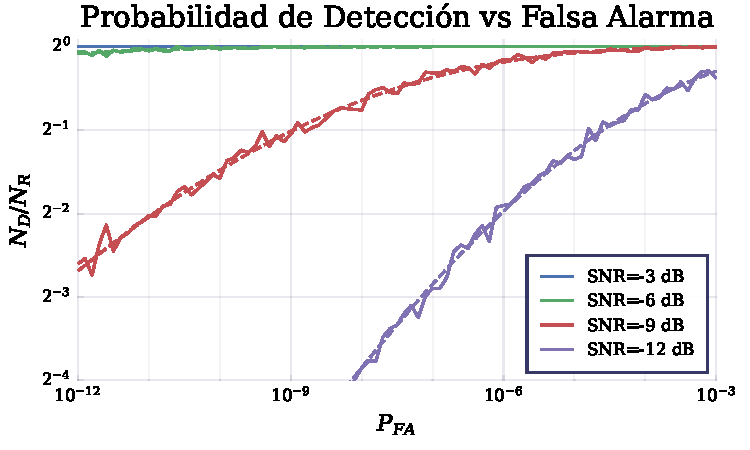
\includegraphics[width=\imsize]{pd_vs_pfa.pdf}
    \caption[Probabilidad de detección en función de la probabilidad de falsa alarma elegida a valores de SNR fijos.]{Resultados de probabilidad de detección de la decisión en función de la probabilidad de falsa alarma elegida a valores de SNR fijos. En línea punteada se grafican los resultados analíticos, y en línea contínua del mismo color los resultados de simulación.\label{fig:pd-vs-pfa}}
\end{figure}
\begin{figure}[t]
    \centering{}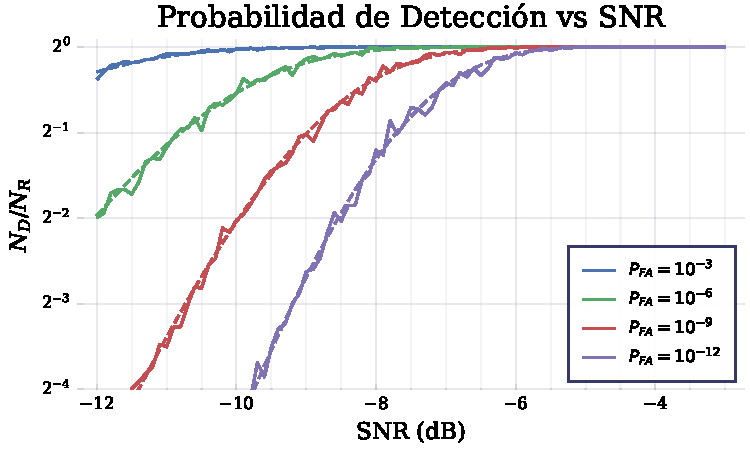
\includegraphics[width=\imsize]{pd_vs_snr.pdf}
    \caption[Probabilidad de detección en función de la SNR elegida a valores de probabilidad de falsa alarma elegida fijos.]{Resultados de probabilidad de detección de la decisión en función de la SNR elegida a valores de probabilidad de falsa alarma elegida fijos. En línea punteada se grafican los resultados analíticos, y en línea contínua del mismo color los resultados de simulación.\label{fig:pd-vs-snr}}  
\end{figure}

\begin{enumerate}
    \item se fijan los valores de $P_{FA}$ y SNR, se determinan arbitrariamente valores de $A$ y $\sigma^2$ que resulten en la SNR elegida al aplicar la Ecuación \ref{eq:snr-definicion}, y se calcula el valor de $T$;
    \item para tener un número de realizaciones razonable, pero estadísticamente representativo del experimento, se elige hacer $100/P_D$ realizaciones;
    \item en cada realización se genera un vector de $N$ muestras $\mathbf{y} = A\mathbf{s}+\mathbf{w}$ con los valores de $A$ y $\sigma^2$ elegidos anteriormente;
    \item se calcula $\phi[\mathbf{y}]$ y se compara el resultado con el valor de $T$, registrando si se produce o no una detección;
    \item una vez terminadas las realizaciones, la probabilidad de detección empírica es el número de detecciones $N_D$ dividido por el número total de realizaciones $N_R$, la cual se compara con el resultado analítico esperado.
\end{enumerate}

Estas simulaciones se ejecutan sobre un vector de valores de SNR manteniendo un valor de $P_{FA}$ fijo, y sobre un vector de valores de $P_{FA}$ manteniendo un valor de SNR fijo. Los resultados de $P_D$ empírico se comparan con las curvas que resultan de evaluar la Ecuación \ref{eq:probabilidad-deteccion-snr}, y se muestran en las Figuras \ref{fig:pd-vs-snr} y \ref{fig:pd-vs-pfa} respectivamente. 

\color{RoyalBlue}
\subsection{Aspectos prácticos para la implementación}

Las hipótesis planteadas para la regla de decisión consideran únicamente la presencia total de la señal de entrenamiento de símbolos cortos o la ausencia total de la misma dentro de la ventana de evaluación. Estas hipótesis facilitan el desarrollo de la regla de decisión, pero no reflejan la totalidad de las situaciones que se encontrarán. 

Una situación que inevitablemente se manifiesta durante la recepción de la trama pero no está contemplada ni en la hipótesis nula ni en la hipótesis alternativa es la presencia parcial de una secuencia de entrenamiento de símbolos cortos. Dada la periodicidad de la secuencia de entrenamiento de símbolos cortos, esto resultará en un incremento en la correlación con la referencia en caso de presencia parcial en la ventana de evaluación, provocando máximos locales los cuales pueden superar el umbral de detección. Este fenómeno se visualiza fácilmente por medio de una simulación en la cual la ventana de evaluación se desplaza sobre una señal que consiste en un preámbulo localizado sobre muestras de ruido aditivo, los resultados de esta simulación se presentan en la Figura \ref{fig:hipotesis-notas}.

Se observa en la Figura un máximo absoluto del estadístico de detección, el cual corresponde al instante en el cual la hipótesis alternativa definida es verdadera. Sin embargo se observan también múltiples máximos locales previos y posteriores a el máximo absoluto, los cuales son producto de la presencia parcial de la secuencia de entrenamiento de símbolos cortos en la ventana, múltiples de los cuales exceden el umbral de detección. Es necesario tomar en cuenta este efecto durante la implementación para evitar detecciones erroneas.

\begin{figure}[t]
    \centering{}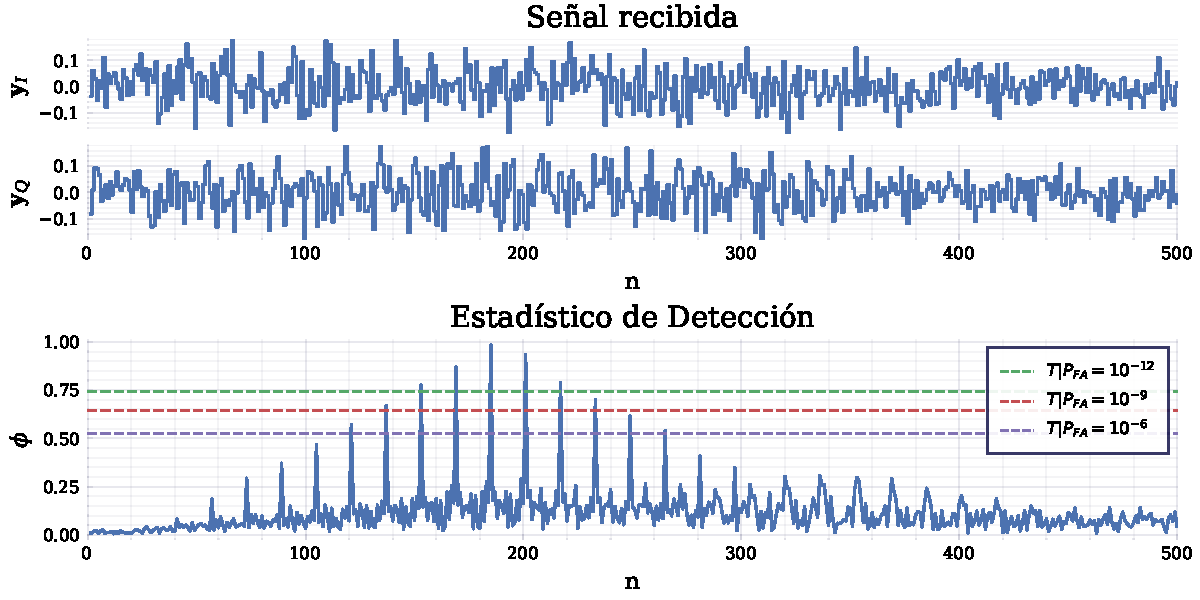
\includegraphics[width=\imsizeL]{hipotesis.pdf}
    \caption[Simulación del estadístico de detección aplicado a una señal recibida que contiene un preámbulo localizado sobre ruido aditivo.]{Simulación del estadístico de detección calculado a partir de ventanas de evaluación secuenciales sobre una señal recibida que contiene un preámbulo localizado sobre ruido aditivo, comparadas contra umbrales de detección que admiten diferentes probabilidades de falsa alarma. La señal bajo simulación se genera con una SNR de 0 dB.\label{fig:hipotesis-notas}}
\end{figure}

\color{black}

\section{Estimación de varianza del ruido}
\label{S:estimacion-ruido}

El problema de detección se definió en función de un umbral que depende de la varianza del ruido, tal como se muestra en la Ecuación \ref{eq:umbral}. Sin embargo, la varianza del ruido es desconocida, y ésta necesita estimarse para poder calcular el umbral. 

Existen varios criterios para elegir un estimador adecuado para el problema, en este caso se elige el estimador insesgado de mínima varianza (MVUE por sus siglas en inglés). Se supone que la estimación del ruido se realiza sobre un vector de muestras que proviene únicamente del ruido, caso que corresponde a la hipótesis nula de la regla de decisión.

\subsection{Cálculo del MVUE de varianza del ruido}
% Para estimar la varianza del ruido, se selecciona el estimador insesgado de mínima varianza (MVUE por sus siglas en inglés). El método para encontrarlo es usando el teorema de Rao-Blackwell-Lehmann-Scheffe. \cite{kay}
% 
% El procedimiento requiere de un estadístico suficiente para un parámetro de la distribución de ciertos datos obtenidos. 
% Los datos se suponen provenientes de ruido normal complejo de media nula independientes e idénticamente distribuidos, se le asigna el nombre $\mathbf{w}$ y su distribución será la siguiente. 
% \begin{equation}\label{eq:noise-estimation-distribution}
%     f(\mathbf{w}) = \frac{1}{\left(2\pi\sigma^2\right)^N} \exp\left[- \frac{\mathbf{w}^\ast \mathbf{w}}{2\sigma^2}\right]
% \end{equation}
% 
% El teorema establece que si uno encuentra una función de un estadístico suficiente que retorne un estimador insesgado del parámetro, este será el MVUE. 
% 
% Para obtener el estadístico suficiente, se utiliza el teorema de factorización de Neyman--Fischer establece que si la distribución de probabilidad de $\mathbf{w}$ puede ser expresada como el producto
% \begin{equation}
%     f(\mathbf{w}, \sigma^2) = g(T(\mathbf{w}), \sigma^2)h(\mathbf{w})
% \end{equation}
% 
% Entonces $T(\mathbf{w})$ es un estadístico suficiente para $\sigma^2$. Efectivamente la distribución tal como es descrita en la ecuación \ref{eq:noise-estimation-distribution} tiene esta forma si se eligen las siguientes funciones
% \begin{equation}
%     h(\mathbf{w}) = 1 \qquad\qquad T(\mathbf{w}) = \mathbf{w}^\ast \mathbf{w}
% \end{equation}
% 
% Para obtener una función de $T(\mathbf{w})$ que retorne un estimador insesgado, resulta util calcular el valor esperado de $T(\mathbf{w})$, lo cual en este caso es fácil ya que las muestras son independientes e idénticamente distribuidas. 
% \begin{equation}
%     E\left[\mathbf{w}^\ast\mathbf{w}\right] =  E\left[\sum_{i=0}^{N-1}\lvert w[i]\rvert^2\right]  =   \sum_{i=0}^{N-1}E\left[\lvert w[i]\rvert^2\right] 
% \end{equation}
% 
% El valor esperado del módulo al cuadrado de una muestra de ruido fue calculado anteriormente, en la Sección \ref{Ss:def-hipotesis}. De esta forma se obtiene el siguiente valor
% \begin{equation}
%     E\left[\mathbf{w}^\ast\mathbf{w}\right] =  \sum_{i=0}^{N-1}2\sigma^2 = 2N\sigma^2 
% \end{equation}
% 
% Conociendo ese valor, puede calcular facilmente una función que retorne un estadístico insesgado aplicando un factor de correción multiplicativo, esta función será el MVUE.
% \begin{equation}
%     \widehat{\sigma^2}_{\text{MVU}} = g\left(\mathbf{w}^\ast\mathbf{w}\right) =  \frac{\mathbf{w}^\ast\mathbf{w}}{2N}
% \end{equation}

El MVUE se puede encontrar utilizando el teorema de la cota inferior de Cramer-Rao \cite{kay}, la cual establece que si la distribución de probabilidad de una variable $\mathbf{x}$ afectada por un parámetro $\theta$ cumple la condición de regularidad,
\begin{equation}
    E\left[\frac{\partial \ln p(\mathbf{x},\theta)}{\partial \theta}\right] = 0,
\end{equation}
y la derivada respecto al parámetro del logaritmo de la distribución de probabilidad de la variable aleatoria se puede factorizar a una expresión del tipo
\begin{equation}\label{eq:cramer-rao}
    \frac{\partial \ln p(\mathbf{x},\theta)}{\partial \theta} = I(\theta)\left(g(\mathbf{x})-\theta\right),
\end{equation}
entonces $g(\mathbf{x})$ será el MVUE para $\theta$. Además, $I(\theta)$ será la información de Fisher de este parámetro, y ésta es inversamente proporcional a la varianza del MVUE,
\begin{equation}\label{eq:var-mvue}
    \text{Var}[\widehat{\theta}_{\text{MVU}}] = \frac{1}{I(\theta)}.
\end{equation}

En este caso el parámetro a estimar es la varianza a partir de un vector de muestras de ruido $\mathbf{w}$, por lo cual $\theta = \sigma^2$, y la distribución de probabilidad de $\mathbf{w}$ queda representada de la forma 
\begin{equation}\label{eq:noise-estimation-distribution}
    f(\mathbf{w}, \theta) = \frac{1}{\left(2\pi\theta\right)^N} \exp\left[- \frac{\mathbf{w}^\ast \mathbf{w}}{2\theta}\right],
\end{equation}
en base a la cual se procede a calcular la derivada respecto al parámetro del logaritmo de la distribución de las muestras, obteniendo la expresión
\begin{equation}\label{eq:logaritmo-derivada}
\frac{\partial \ln p(\mathbf{w},\theta)}{\partial \theta} =  - \frac{N}{ \theta} +\frac{\mathbf{w}^\ast\mathbf{w}}{2\theta^2}.
\end{equation}

La condición de regularidad se puede verificar fácilmente, al considerar que las muestras son independientes e identicamnte distribuidas. A su vez, la Ecuación \ref{eq:logaritmo-derivada} se puede factorizar de forma
\begin{equation}\label{eq:logaritmo-derivada-factorizacion}
    \frac{\partial \ln p(\mathbf{w},\theta)}{\partial \theta} =  \frac{N}{\theta^2}\left(\frac{\mathbf{w}^\ast\mathbf{w}}{2N}-\theta\right),
\end{equation}
la cual es consistente con la Ecuación \ref{eq:cramer-rao}, y nos da el MVUE y la información de Fisher:
\begin{equation}\label{eq:expresion-mvue}
    \widehat{\sigma^2}_{\text{MVU}} = \frac{\mathbf{w}^\ast\mathbf{w}}{2N}, \qquad\qquad I(\sigma^2) = \frac{N}{\left(\sigma^2\right)^2}.
\end{equation}
% El valor esperado del módulo al cuadrado de una muestra de ruido fue calculado anteriormente, en la Sección \ref{Ss:def-hipotesis}. De esta forma se obtiene el siguiente valor
% \begin{equation}
%     E\left[\mathbf{w}^\ast\mathbf{w}\right] =  \sum_{i=0}^{N-1}2\sigma^2 = 2N\sigma^2 
% \end{equation}

\subsection{Desempeño del estimador}
\label{Ss:estimador-ruido-desempeño}

%\begin{equation}  
%    \begin{aligned}
%        \ln p(\mathbf{w},\sigma^2) &= - N \ln\left[2\pi \sigma^2\right]-\frac{\mathbf{w}^\ast\mathbf{w}}{2\sigma^2}\\
%        \frac{\partial \ln p(\mathbf{w},\sigma^2)}{\partial \sigma^2} &=  - \frac{N}{ \sigma^2} +\frac{\mathbf{w}^\ast\mathbf{w}}{2\left(\sigma^2\right)^2}\\
%        \frac{\partial^2 \ln p(\mathbf{w},\sigma^2)}{\partial \left(\sigma^2\right)^2} &=   \frac{N}{\left(\sigma^2\right)^2}-  \frac{\mathbf{w}^\ast\mathbf{w}}{\left(\sigma^2\right)^3}
%    \end{aligned}
%\end{equation}
 
La métrica utilizada para evaluar el desempeño del estimador será el error cuadrático medio, definido de la siguiente forma
\begin{equation}\label{eq:mse-def}
    \text{MSE}[\widehat{\theta}] = E\left[(\widehat{\theta}-\theta)^2\right] = \text{Var}[\widehat{\theta}] + b^2[\widehat{\theta}],
\end{equation}
donde $b[\widehat{\theta}]$ es el sesgo del estimador. En el caso de los estimadores insesgados como lo es el MVUE, el error cuadrático medio es igual a la varianza del estimador. La varianza del MVUE fue calculada teóricamente a partir de la cota inferior de Cramer-Rao y se Ecuación \ref{eq:var-mvue}, por lo que el error cuadrático medio teórico del estimador es conocido
\begin{equation}\label{eq:mvue-mse}
    \text{MSE}[\widehat{\sigma^2}_{\text{MVU}}] = \frac{\left(\sigma^2\right)^2}{N}.
\end{equation}
El desempeño del MVUE se valida calculando el error cuadrático del mismo sobre realizaciones de ruido con varianza conocida, y se verifica que este tenga el comportamiento esperado. Este resultado se presenta en la Figura \ref{fig:estimator_mse}.
\begin{figure}[t]
    \centering{}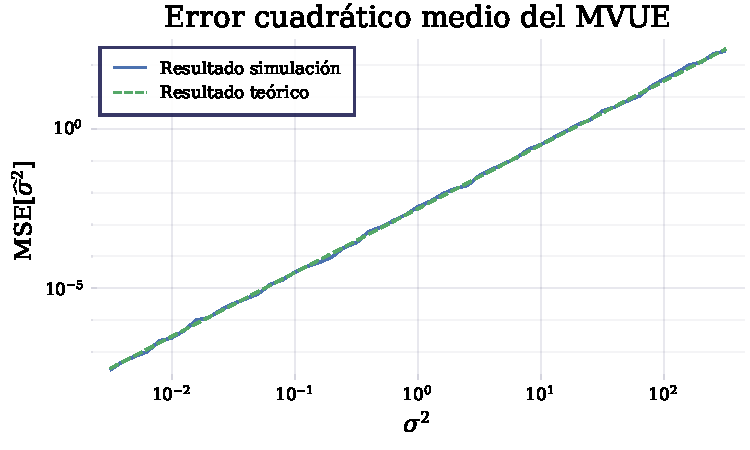
\includegraphics[width=\imsize]{estimator_mse.pdf}
    \caption[Error cuadrático medio del MVUE para la varianza del ruido.]{Resultados de la verificación por simulación del error cuadrático medio del MVUE para la varianza del ruido.\label{fig:estimator_mse}}
\end{figure}

En principio, se podría estimar el ruido a partir de las mismas muestras que se utilizan para calcular $\phi$. Sin embargo, estas muestras no siempre van a cumplir la suposiciones que se planetaron para derivar la expresión del MVUE, las cuales implicaban que la hipótesis nula es verdadera. Se procede a evaluar numéricamente si el error cuadrático medio del estimador incrementa al aplicar el mismo ante la hipótesis alternativa. 

Ese ensayo se logra generando múltiples realizaciones de un vector $\mathbf{y}$ que consistan en una secuencia de entrenamiento de símbolos cortos más ruido con determinada SNR, calculando el MVUE expresado en la Ecuación \ref{eq:expresion-mvue} en en esas condiciones, y promediando el error cuadrático. \color{RoyalBlue} Para independizar la medida del error cuadrático medio de la varianza utilizada para generar las muestras de ruido evidenciada por la Ecuación \ref{eq:mvue-mse}, se define el error cuadrático medio normalizado,
\begin{equation}
    \text{MSE}_N[\widehat{\sigma^2}_{\text{MVU}}] = \frac{\text{MSE}[\widehat{\sigma^2}_{\text{MVU}}]}{\left(\sigma^2\right)^2}.
\end{equation}
A fin de estudiar los factores que contribuyen al error cuadrático medio evidenciados por la Ecuación \ref{eq:mse-def}, el sesgo y la varianza del estimador, se definen el sesgo normalizado y la varianza normalizada,
\begin{equation}
    b_N[\widehat{\sigma^2}_{\text{MVU}}] = \frac{b[\widehat{\sigma^2}_{\text{MVU}}]}{\sigma^2},
    \quad
    \text{Var}_N[\widehat{\sigma^2}_{\text{MVU}}] = \frac{\text{Var}[\widehat{\sigma^2}_{\text{MVU}}]}{\left(\sigma^2\right)^2}.
\end{equation}
Estos factores se calculan por simulación y se comparan con el error cuadrático medio. Los resultados de las simulaciones realizadas se muestran en la Figura \ref{fig:estimator_mse_snr}.
\begin{figure}[t]
    \centering{}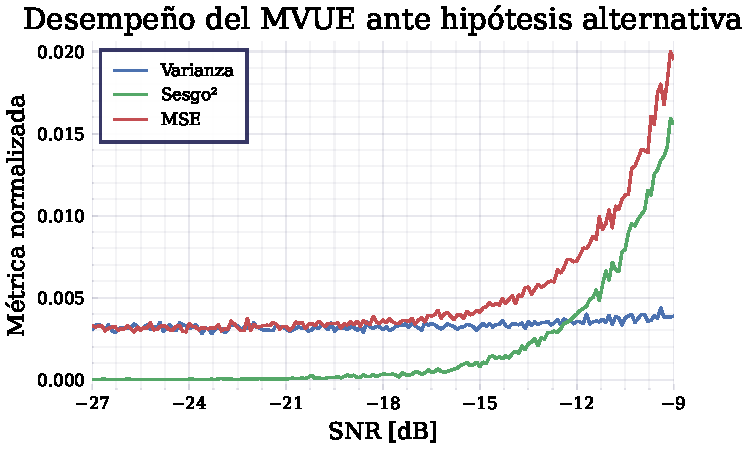
\includegraphics[width=\imsize]{estimator_mse_snr.pdf}
    \caption[Degradación del MSE normalizado del MVUE para la varianza del ruido ante presencia de señales en la ventana de evaluación.]{Resultados de simulación numérica del error cuadrático medio normalizado, sesgo normalizado, y varianza normalizada del MVUE para la varianza del ruido ante la presencia de una secuencia de entrenamiento de símbolos cortos con determinada SNR en la ventana de muestras utilizadas para calcular el estadístico..\label{fig:estimator_mse_snr}}
\end{figure}
\color{black}

Se determina que la estimación del ruido será incorrecta cuando la hipótesis alternativa sea verdadera, este fenómeno afectaría el cálculo del umbral si no se tomara en cuenta. La estrategia para evitar este efecto es simple cuando se consideran las propiedades de la transmisión. Se sabe que el preámbulo se recibe al inicio de cualquier señal OFDM, previo a éste no existe señal. Teniendo en cuenta esto, basta utilizar muestras pasadas para estimar el ruido y calcular el umbral contra el cual se comparará el estadístico de detección actual para la regla de decisión.


\color{Green}
\section{Implemetación en LabVIEW}

Dado que el estadístico de detección utilizado se puede obtener a partir del funcional del banco de correladores ya implementado y descrito en la Sección \ref{Ss:ch3-labview}, no hay necesidad de calcularlo nuevamente. Se requiere únicamente implementar la obtención del MVUE para la varianza del ruido y el cálculo del umbral de detección. 

De la misma forma que los funcionales de sincronismo, el MVUE se calcula a partir de las muestras en una ventana de evaluación $\mathbf{v}$, el diagrama de bloques que la implementa se presenta en la Figura \ref{fig:noise-est-lv}. El MVUE calculado junto con la probabilidad de falsa alarma elegida y la norma de la secuencia de entrenamiento de símbolos cortos se utilizan de forma directa para calcular el umbral de detección por medio del diagrama de bloques presentado en la Figura \ref{fig:threshold-lv}.

\begin{figure}[t]
    \centering
    \hfill
    \subcaptionbox{Cálculo del MVUE para la varianza del ruido.\label{fig:noise-est-lv}}{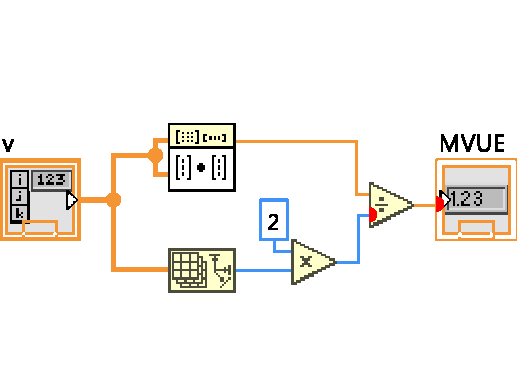
\includegraphics[width=0.5\imsizeL]{xpstopdf/noise-est-lv.pdf}}%
    \hfill
    \subcaptionbox{Cálculo del umbral de detección.\label{fig:threshold-lv}}{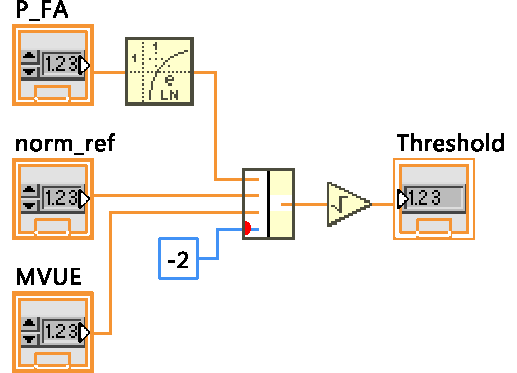
\includegraphics[width=0.5\imsizeL]{xpstopdf/threshold-lv.pdf}}%
    \caption{Diagramas en bloques de las implementaciones en LabVIEW de las operaciones necesarias para el algoritmo de detección.\label{fig:deteccion-lv}}
    \hfill
\end{figure}

\subsection{Complejidad computacional de la implementación}
La estimación de la varianza del ruido incorpora un producto interno, por lo que esta operación es de orden de complejidad $\mathcal{O}(N)$. El cálculo del umbral de detección definido en la Ecuación \ref{eq:umbral} incluye la norma de la referencia, la cual también es un producto interno, pero es posible precalcularla por lo que no es necesario considerarla para el análisis de complejidad computacional. Las operaciones restantes incluyen el logaritmo y la raiz cuadrada, las cuales requieren múltiples operaciones de punto flotante pero mantienen orden de complejidad $\mathcal{O}(1)$.
 
\color{black}

\section{Resumen del capítulo}

Se formalizaron las hipótesis mutuamente excluyentes acerca de la composición de las muestras de la señal recibida: una hipótesis nula que corresponde a la ausencia de una señal entrante; y una hipótesis alternativa que corresponde a la presencia de la misma. En el caso de que exista una señal entrante, se definió una medida de relación señal a ruido.  

En función de las muestras recibidas se definió un estadístico y una regla de decisión en base a un umbral contra el cual se compara el estadístico elegido para discriminar entre las hipótesis. Se definieron la probabilidad de detección y la probabilidad de falsa alarma, esta última se usó para elegir el valor del umbral, y se analizó cómo la probabilidad de falsa alarma elegida y la SNR afectan a la probabilidad de detección. 

Finalmente, se encontró el estimador insesgado de mínima varianza para la varianza del ruido, el cual será necesario para definir el umbral de la regla de decisión. Se observó que la presencia de señales en las muestras recibidas afecta el desempeño de este estimador, por lo que se propone resolver este problema por medio de un desfasaje temporal en la ventana que se utiliza para estimar la varianza del ruido y la ventana sobre la cual se aplica la regla de decisión.
